\documentclass[a4paper, 14pt]{extarticle}
\usepackage[left=2cm,right=2cm,top=2cm,bottom=2cm,bindingoffset=0cm]{geometry}
\usepackage[utf8]{inputenc}
\usepackage[english, russian]{babel}
\usepackage{amssymb, latexsym, amsmath}
\usepackage{indentfirst}
\usepackage{graphicx}
\usepackage{citehack}
\usepackage{tabularx}
\usepackage{listings}
\usepackage{pdfpages}

\lstloadlanguages{HTML,python}
\lstset{extendedchars=false,
  breaklines=true,
  breakatwhitespace=true,
  keepspaces = true,
  tabsize=2
}


\begin{document}
\begin{titlepage}

\newpage

\begin{center}
Московский Авиационный Институт \\*
(национальный исследовательский университет) \\*

\vspace{2em}

Факультет прикладной математики и физики \\*
Кафедра вычислительной математики и программирования

\vspace{10em}

\Large \textbf{Курсовой проект \\*
по дисциплине <<Информационные технологии в проектировании и производстве>>} \\*

\vspace{3em}

<<Разработка проектного офиса <<Цифромед>>
\end{center}

\vspace{8em}

\hspace{25em}\vbox{
  \hbox{\bfseries{Выполнил:}}
  \hbox{\hspace{1em} Данилычев И.\,А.}
}

\vspace{2em}

\hspace{25em}\vbox{
  \hbox{\bfseries{Руководитель:}}
  \hbox{\hspace{1em} Скородумов С.\,В.}
}

\vspace{\fill}

\begin{center}
Москва, 2015
\end{center}

\end{titlepage}

\newpage


\tableofcontents
\newpage


\section{Аннотация}
При компании <<Скородумов и Партнеры>> был сформирован отдел проектирования программного обеспечения, специализирующийся на создании интернет-решений для малого и среднего бизнеса, образовательных учреждений, госпредприятий, задачей которого стала разработка офиса управления проектами, позиционирующегося как SaaS-приложение (Software as a Service, или <<ПО как услуга>>).

Результатом работы над проектом стало появление на свет проектного офиса <<Цифромед>>, представленного в виде веб-приложения, реализованного на языке Python с применением многофункционального фреймворка Flask.

Одной из целей проекта также являлось обеспечение компании <<Скородумов и Партнеры>> решением для управления проектами, предназначенным для внутреннего пользования и при этом, несмотря на имеющиеся аналоги (teamtools.ru, <<Мегаплан>> и др.), не уступающим им по основным показателям производительности и функциональности.


В данный отчёт входят:

\begin{itemize}
\setlength{\itemsep}{-1mm}
\item Иерархическая модель работ (WBS, Work Breakdown Structure) и бизнес-модель проекта;
\item IDEF0-модель цикла разработки данного проекта;
\item Техническое задание;
\item Структура базы данных приложения;
\item Описание модели разработки;
\item Программная логика серверной части (backend);
\item Описание интерфейсной части (frontend);
\item Паспорт проекта и его данные.
\end{itemize}

\newpage


\section{Анализ проекта}
\subsection{Цель проекта}

Ни для кого не секрет, что грамотное планирование в совокупности с тайм-менеджментом и распределением ответственности, зачастую реализуемым через методологию иерархической структуры проекта (Work Breakdown Structure), являются <<сердцем>> любого проекта и в основном определяют успешность его жизненного цикла вкупе с полнотой.

Целью данного проекта являлось создание веб-сервиса, оформленного в виде SaaS-решения и имеющего достаточно возможностей для замещения собой сторонних аналогов. Полученный продукт возможно как применять для внутреннего пользования, так и вывести на рынок ПО для последующей монетизации.

\subsubsection{Достижимость цели}
Несмотря на поставленную цель, проектная команда во главе с проект-менеджером отдаёт себе отчёт в том, что полученный результат может не содержать в себе всех заявленных особенностей, требуемых для успешной конкуренции со сторонними разработками. Более того, он может проигрывать по качеству исполнения и набору имеющихся или планируемых возможностей, которыми обладают коммерческие решения, созданные командами большого размера.
	
	
\subsection{Продукт проекта}

Для успешной реализации задач, поставленных в цели проекта, используется концепция проектного офиса, компонента, где происходит координация, обобщение информации и централизация прикрепленных проектов, ведется сводный мониторинг бюджетов и графиков. Проектный офис также обеспечивает коммуникацию между различными рабочими группами и скоординированную работу менеджеров проектов.

Проектный офис чаще всего, как и в данной работе, реализуется в виде Software as a Service-услуги, или, проще говоря, Web-приложения, не требующего установки на клиентские компьютеры. Всё, что требуется от членов проекта -- наличие доступа ко внутренней иерархии системы (комбинация логина и пароля), остальное же обеспечивается подразделением, ответственным за настройку и администрирование программных и аппаратных ресурсов организации.


\subsection{Work Breakdown Structure}
Work Breakdown Structure, или структура декомпозиции работ -- это иерархическое разбиение всей работы, которую необходимо выполнить для достижения целей проекта, на более мелкие операции и действия до такого уровня, на котором способы выполнения этих действий вполне ясны, а соответствующие работы могут быть оценены и спланированы. Она включает также определение промежуточных результатов всех составляющих эту структуру работ.

WBS чаще всего выполнена в виде древовидной диаграммы, корневым узлом в которой является сам проект, а его дочерними узлами -- результаты и подрезультаты, требуемые для достижения целей проекта. Важно отметить, что, помимо определения всего объёма работ для проекта, каждый из узлов структуры декомпозиции представляет собой объективный или как минимум измеримый результат.

Work Breakdown Structure используется для разделения ответственности и выделения конкретного набора обязанностей, которыми обладает каждая из рабочих групп и каждый сотрудник в отдельности. WBS для настоящего проекта приведена ниже:


\vspace{1em}

\begin{figure}[!htb]
  \centering
    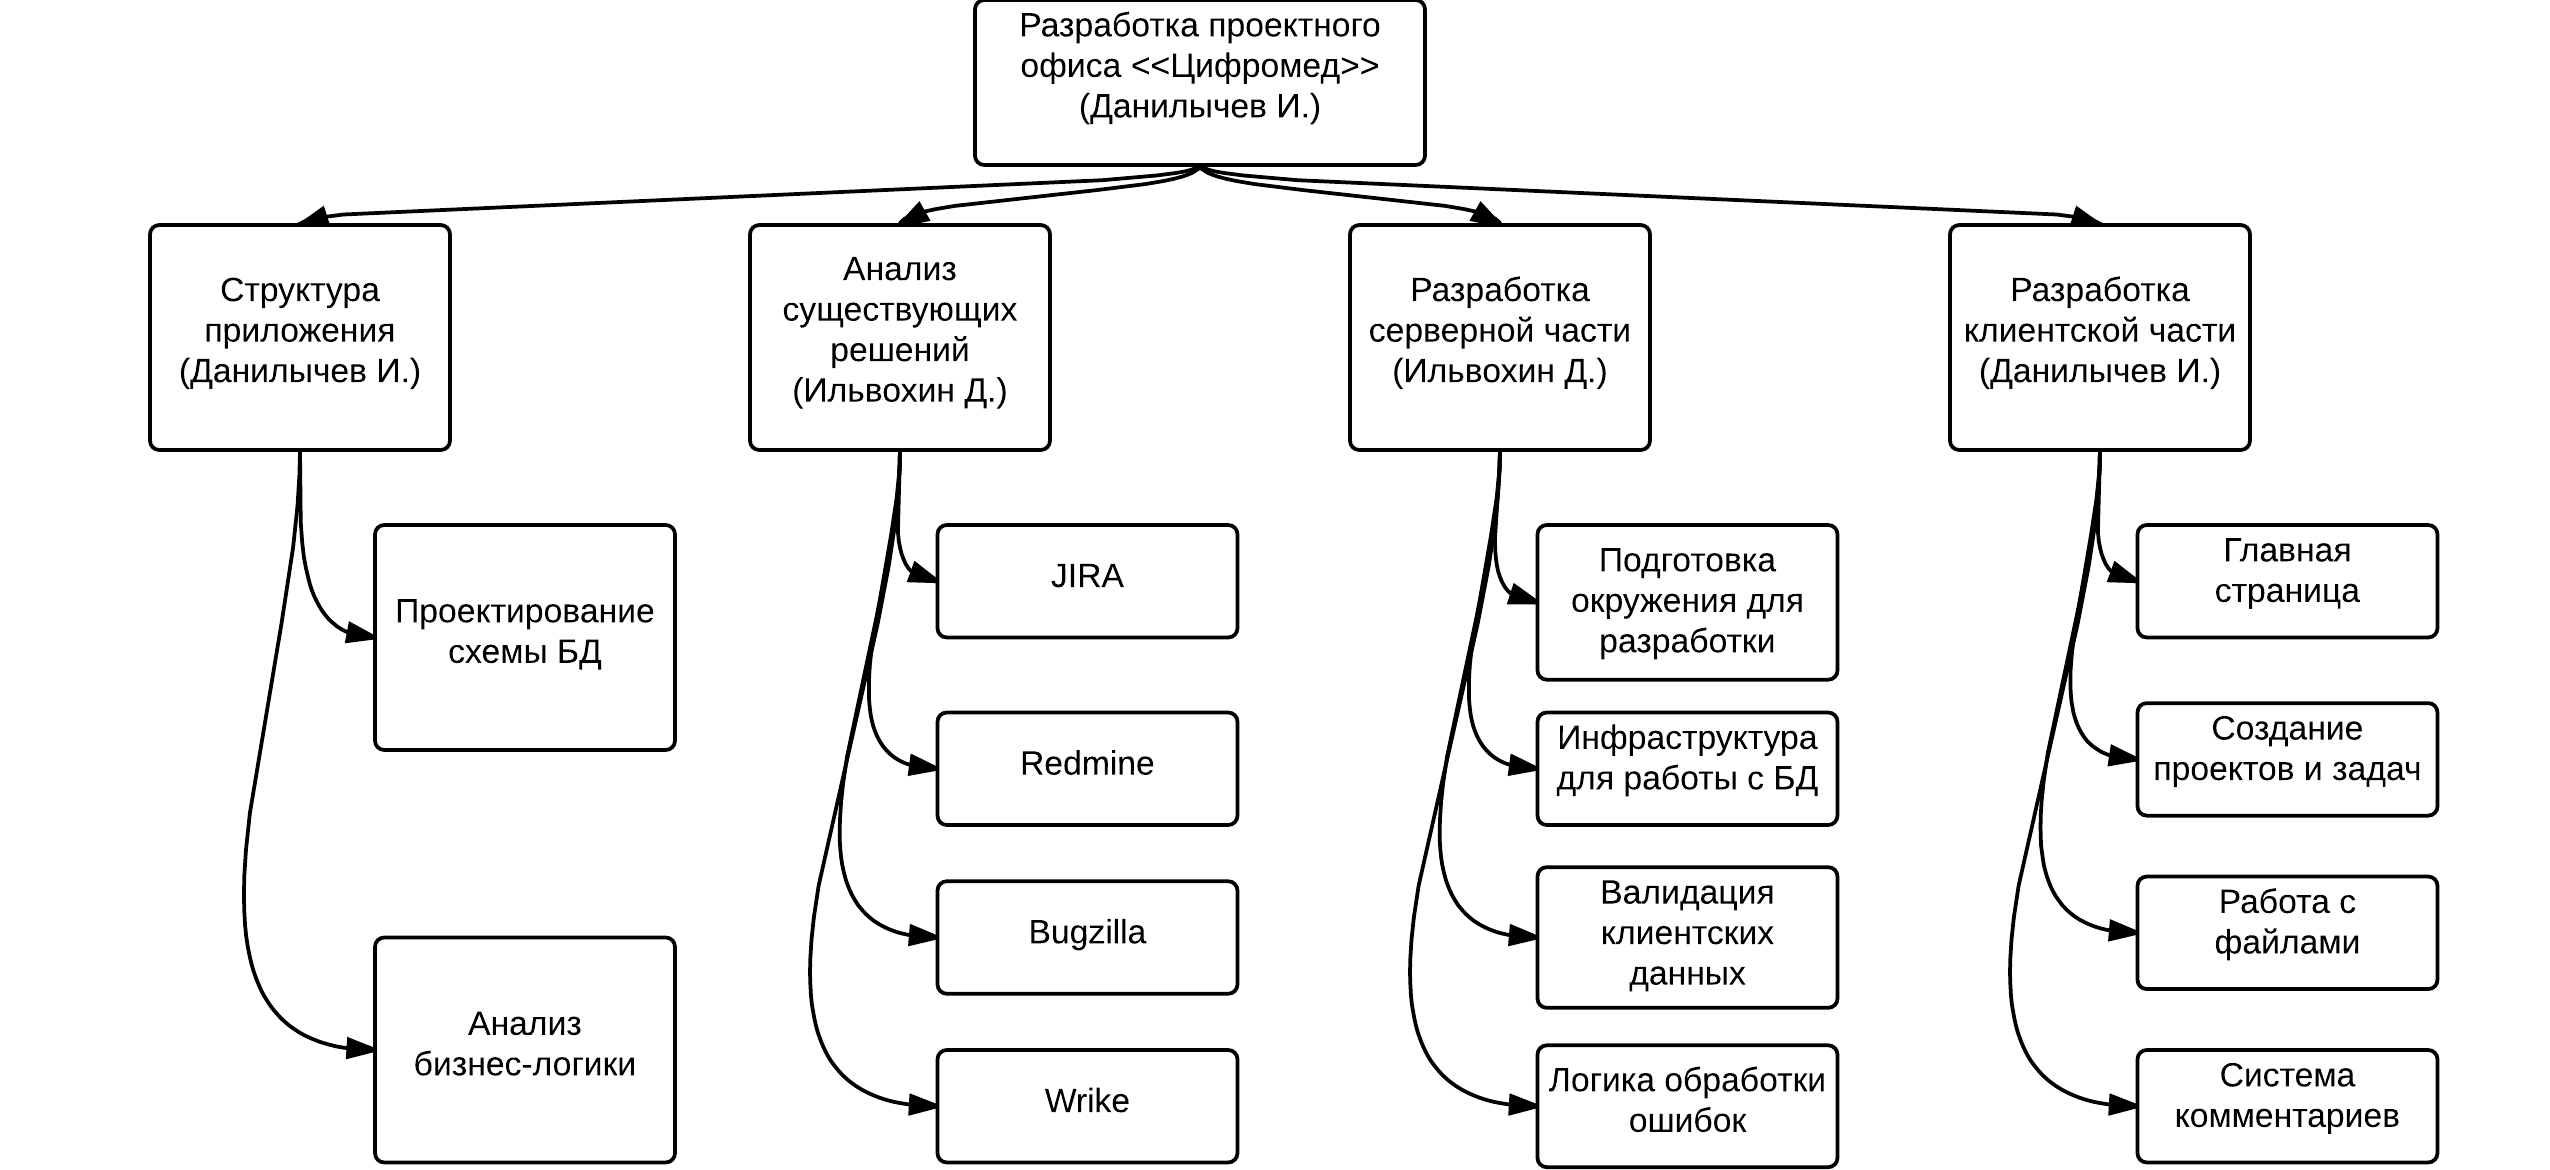
\includegraphics[scale=0.25]{../shared_images/wbs.png}
   \caption{Структура декомпозиции работ}
    \label{fig:start}
\end{figure}
\newpage


\subsection{Бизнес-модель проекта}

\begin{figure}[!htb]
  \centering
    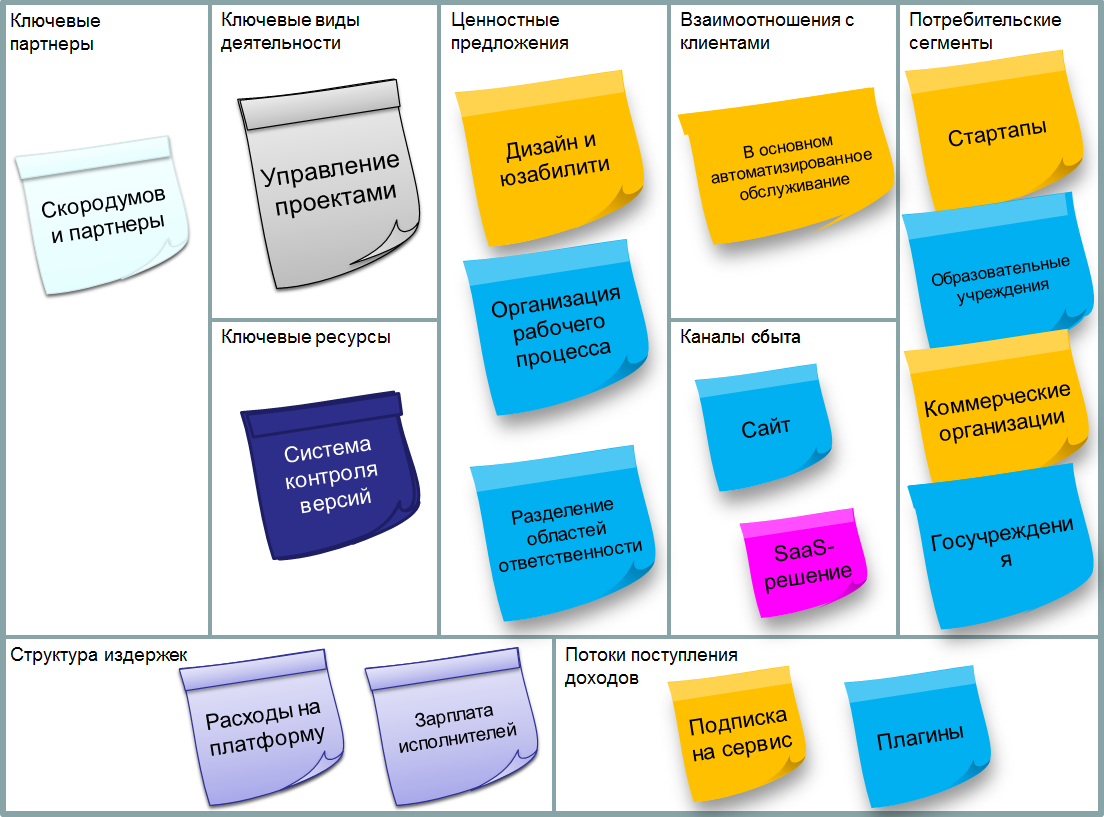
\includegraphics[scale=0.6]{../shared_images/business-model.png}
   \caption{Бизнес-модель проекта}
    \label{fig:start}
\end{figure}
  
Как видно из вышеприведённой модели, ключевым ресурсом проекта является децентрализованная система контроля версий. % Дописать про гит/гитхаб

В потребительские сегменты попали коммерческие, государственные и образовательные организации, а также стартапы. Потребители (клиенты) – сердце любой бизнес-модели. Без (выгодных) клиентов не может существовать ни одна компания. Чтобы лучше удовлетворять нужды клиентов, желательно разбить их на группы по потребностям, особенностям поведения или иным признакам. Так, для образовательных организаций стоит делать упор на низкую себестоимость данного решения, его простоту в освоении, доступность и пр.

Взаимоотношения с клиентами, благодаря самобалансируемости и самоподдерживаемости проекта, сводятся к минимуму; что же касается сервиса поддержки клиентов, он относится к вопросам монетизации (поступление доходов).

Ценностные предложения сводятся к реализации функций, описанных в цели проекта: организации рабочего процесса и взаимодействия проектных команд и членов проектов, разделения сфер ответственности и т.д., а также простому, минималистичному дизайну, который в данном случае, учитывая порой переусложнённые интерфейсы конкурентов, является скорей положительным фактором.

Создание и воплощение ценностных предложений, поддержание взаимоотношений с потребителями, получение прибыли – все эти процессы связаны с какими-либо издержками. Расходы достаточно легко подсчитать при уже определённых ключевых ресурсах, видах деятельности. В данном случае издержки сводятся к оплате труда программистов, работавших над проектным офисом, и расходам на поддержание офиса в рабочем состоянии (оплата хостинга и т.п.)

Наконец, потоки поступления доходов в данной модели представлены двумя возможностями. Первая -- продажа подписки на сервис поддержки клиентов, который будет обеспечивать техническое функционирование офиса на клиентской стороне (аналогичный подход используется многими компаниями, поставляющими SaaS-услуги, напр., Redmine). Вторая -- разработка встраиваемых компонент, или плагинов, по техническому заданию заказчика, которому недостает в стандартной поставке решения некоторых возможностей.

\newpage


\subsection{IDEF0}
IDEF0 -- методология функционального моделирования и графическая нотация, предназначенная для формализации и описания бизнес-процессов. Отличительной особенностью IDEF0 является её акцент на соподчинённость объектов. В IDEF0 рассматриваются логические отношения между работами без учёта временной последовательности; таким образом, описание workflow, или потока работ, остаётся за рамками данной модели.

\vspace{1em}

\begin{figure}[!htb]
  \centering
    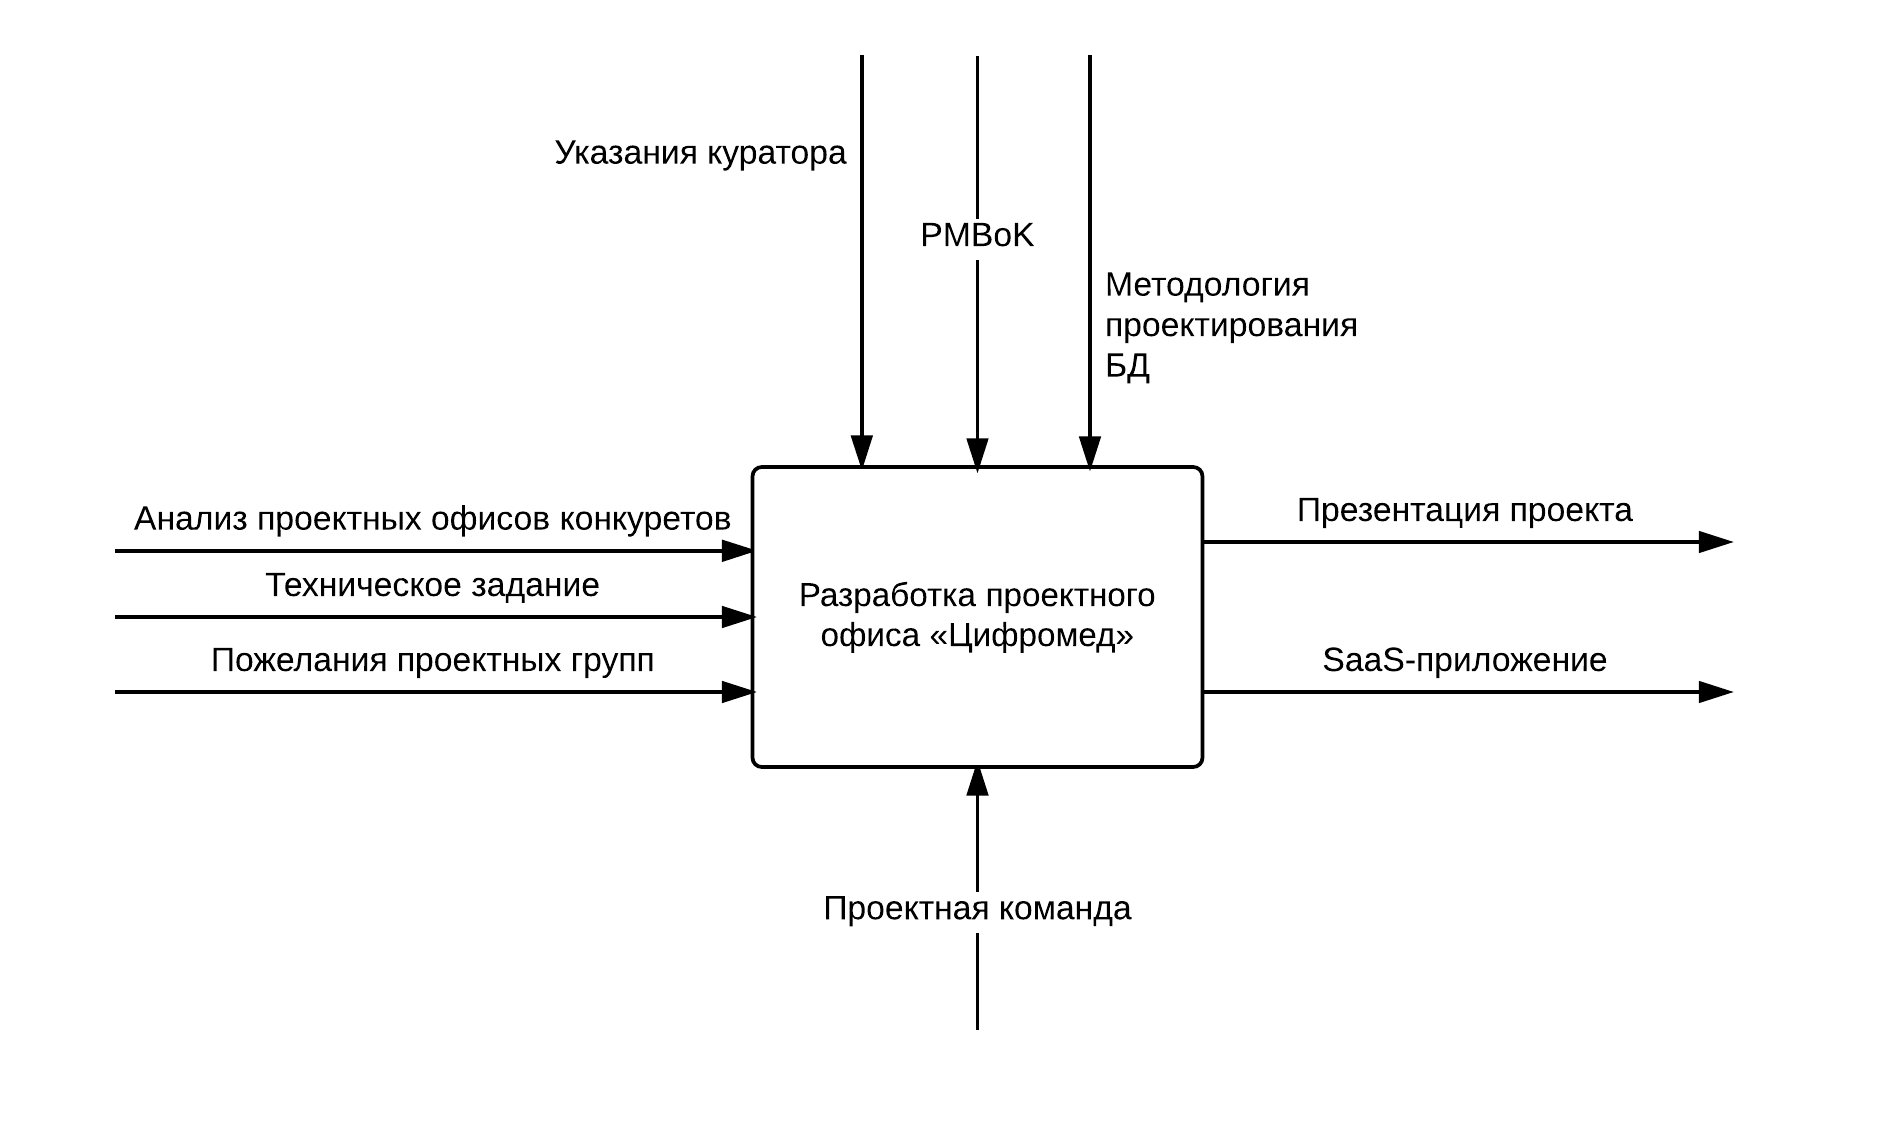
\includegraphics[scale=0.35]{../shared_images/idef0.png}
   \caption{IDEF0-диаграмма}
    \label{fig:start}
\end{figure}

Как видно из приведённой диаграммы, входными данными в настоящем проекте являются данные, полученные при анализе проектных офисов конкурентов, таких как JIRA, Redmine, Bugzilla, а также сформулированное самими разработчиками техническое задание, основанное на предъявляемых к системе требованиях. Кроме того, при разработке учитывались пожелания целевой аудитории, а именно -- проектных групп, являющихся потенциальными клиентами.

При разработке проектного офиса использовались указания куратора, Скородумова С.В., и материалы американского национального стандарта PMBoK, представляющего из себя сумму профессиональных знаний по управлению проектами.

Выходные данные представлены SaaS-приложением, реализующим онлайн-систему управления проектами (проектный офис), и презентацией получившегося продукта.

Декомпозированный уровень IDEF0 приведён ниже:

\vspace{1em}

\begin{figure}[!htb]
  \centering
    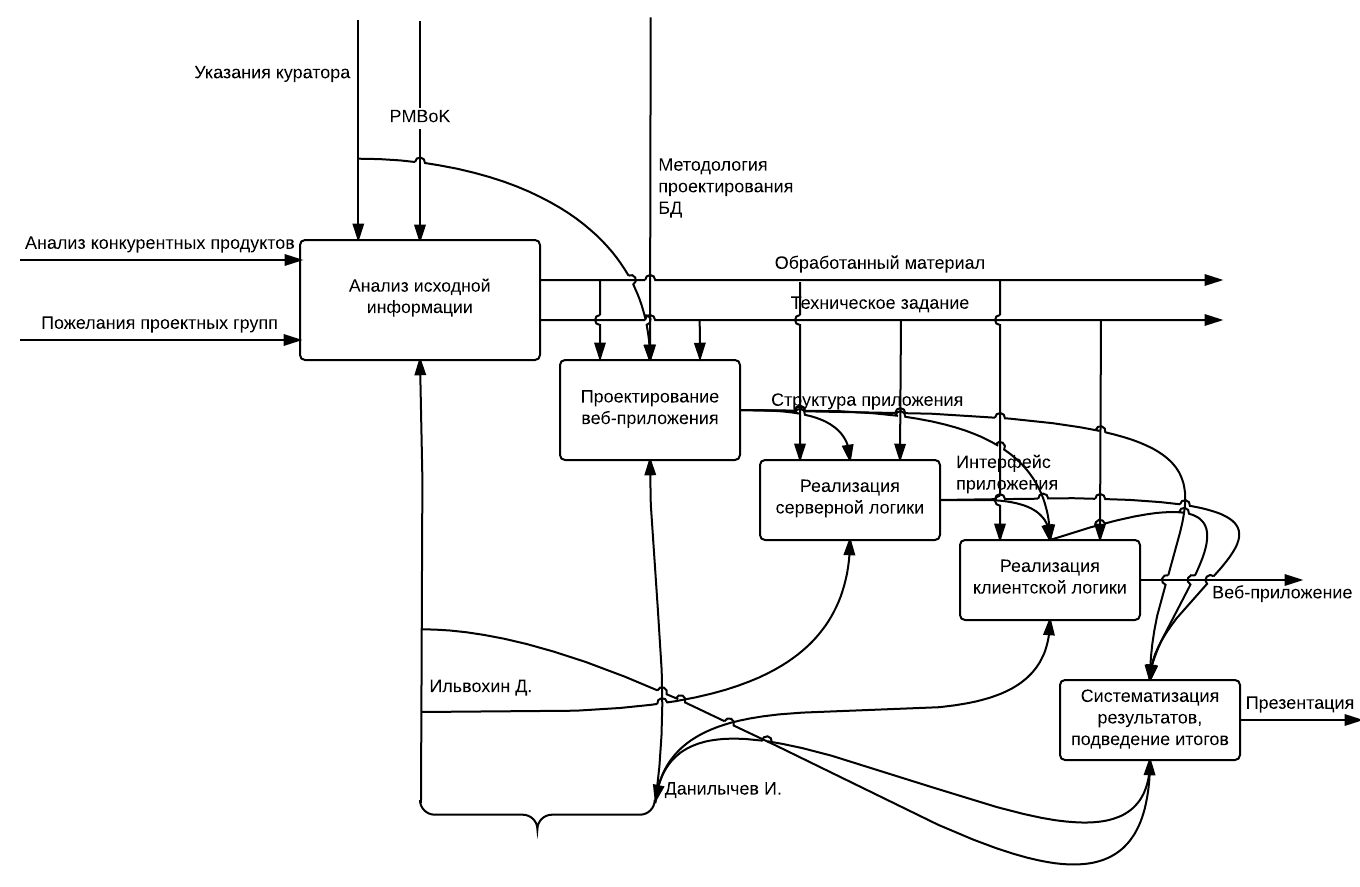
\includegraphics[scale=0.45]{../shared_images/idef0-decomposed.png}
   \caption{Декомпозированный уровень IDEF0}
    \label{fig:start}
\end{figure}

Из него видно, что после обработки конкурентных продуктов и пожеланий проектных групп появляются обработанный и систематизированный материал, который применяется во всех остальных стадиях жизненного цикла проекта, и техническое задание, служащее основой для построения схемы базы данных приложения и его общей системной структуры. Также оба компонента являются определяющими при реализации бизнес-логики на стороне клиента и сервера и применяются при подготовке финальной презентации, являющейся, в свою очередь, одним из продуктов проекта.

\newpage


\section{Техническое задание}
% Краткая аннотация, а затем -- задание из репозитория (с небольшими переработками)

\newpage


\section{Структура приложения}
  \subsection{Схема базы данных}
  % Описание, <<как пришли>> и схема
  
  \subsection{Бизнес-логика}
  % Много из http://habrahabr.ru/post/65432/
  
\newpage


\section{Сравнение существующих решений}
Управление проектами --- в соответствии с определением национальным стандартом
ANSI PMBoK — область деятельности, в ходе которой определяются и достигаются
четкие цели проекта при балансировании между объёмом работ, ресурсами 
(такими как деньги, труд, материалы, энергия, пространство и др.), временем, качеством и рисками. 
Ключевым фактором успеха проектного управления является наличие чёткого заранее определённого плана,
минимизации рисков и отклонений от плана, эффективного управления изменениями.~\cite{wiki_pm}

\subsection{Задачи программного обеспечения для управления проектами}
Для достижения конечных целей проекта менеджеру проекта необходимо специальное программное обеспечение
для управления проектом или портфелем проектов.
Задачи программного обеспечения такого рода обычно делят на три части:
\begin{itemize}
  \item планирование;
  \item управление данными и предоставление информации;
  \item управление коммуникациями команды проекта.
\end{itemize}

\subsubsection{Планирование}
Одной из наиболее распространенных и на мой взгляд наиболее важных возможностей
программного обеспечения для управления проектами является возможность планирования
событий и управления задачами. Требования могут различаться в зависимости от того
для каких целей и проектов используется инструмент, наиболее распространенными являются:
\begin{itemize}
  \item планирование различных событий, зависящих друг от друга;
  \item планирование расписания работы сотрудников и назначение ресурсов на конкретные задачи;
  \item расчет времени, необходимого на решение каждой из задач;
  \item сортировка задач в зависимости от сроков их завершения;
  \item управление нескольким проектами одновременно.
\end{itemize}

\subsubsection{Управление данными и предоставление информации}
Программное обеспечение для управления проектами предоставляет большое количество
требуемой информации, такой как:
\begin{itemize}
  \item список задач для сотрудников и информацию распределения ресурсов;
  \item обзор информации о сроках выполнения задач;
\end{itemize}

\subsubsection{Управление коммуникациями команды проекта}
\begin{itemize}
  \item обсуждение и согласование рабочих вопросов проекта;
  \item предоставление доступа к информации о ходе проекта в виде живой ленты событий.
\end{itemize}

\subsection{Типы программного обеспечения для управления проектами}
Выделяют два типа программного обеспечения по размещению:
\begin{itemize}
  \item desktop (настольные);
  \item web-based (веб-приложения).
\end{itemize}

А также три типа по количеству пользователей использующих приложения:
\begin{itemize}
  \item персональные;
  \item однопользовательские;
  \item многопользовательские.
\end{itemize}

\subsection{Сводная таблица}
Для сравнения программного обеспечения для управления проектами было выделено
несколько пунктов:
\begin{enumerate}
\item Лицензия. Для использования приложения необходимо заплатить деньги
  его разработчикам, если это проприетарное программное обеспечение, как правило,
  при такой лицензии самостоятельная доработка продукта невозможна, потому
  что авторы приложения не распространяют его исходные коды или распространяют, но
  явно запрещают его изменение. При свободной лицензии,
  напротив, возможна самостоятельная доработка.
\item Язык реализации. У некоторых языков программирования, для больших приложений
  большой оверхед использования ресурсов, соответственно для развертывания приложения
  потребуется больше дорогих вычислительных мощностей.
\item Интерфейс. Чем больше возможностей доступа к приложению имеет пользователь --- тем лучше.
  Как правило, удобство использования приложения это первое на что обращает внимание пользователь,
  и в зависимости от своего впечатления делает выбор в пользу какого-то приложения.
\item База данных. Нам как разработчикам приложения было интересно, на основе каких баз данных
  работают существующие/популярные системы, поэтому этот пункт тоже был включен в сравнительную таблицу.
\end{enumerate}

\begin{table}[!htb]
  \caption{Сравнение систем управления проектами~\cite{jira_off}~\cite{redmine_off}~\cite{bugzilla_off}~\cite{wrike_off}}
  \label{tab:cmp_pm}
  \begin{center}
    \begin{tabularx}{\textwidth}{|l|X|X|X|X|}
      \hline
      Система & Лицензия & Язык реализации & Интерфейс & БД \\
      \hline
      JIRA & проприетарное ПО & Java & Web, e-mail, RSS & MySQL, Oracle, PostgreSQL, MS SQL Server и др. \\
      \hline
      Redmine & GPL v2 & Ruby on Rails & Web, E-mail, Atom, iPhone, Windows Phone, Android & MySQL, PostgreSQL, SQLite \\
      \hline
      Bugzilla & MPL & Perl & Web, e-mail, RSS, Web service, cli, iPhone & MySQL, PostgreSQL \\
      \hline
      Wrike & проприетарное ПО & Java & Web, email & PostgreSQL \\
      \hline
      Цифромед & свободная & Python & Web & CouchDB \\
      \hline
    \end{tabularx}
  \end{center}
\end{table}

Для полноты сравнения в таблицу~\ref{tab:cmp_pm} добавлено приложение, разработанное нами.

\newpage

\section{Подготовка окружения для разработки}
Для совместной разработки проекта была выбрана децентрализованная система контроля
версий --- git, которая была создана Линусом Торвальдсом для управления разработкой
ядра Linux.~\cite{git_home}

Для разработки проекта было решено не поднимать git на собственном сервере, а использовать
готовую платформу Github.

При разработке системы решили использовать модель разработки, предложенную Винсентом
Дрессэнем (англ. Vincent Driessen).~\cite{git_branching_model}

Основной идеей этой модели разработки является то, что все изменения происходят в
<<develop>> ветке, от которой (когда разработка всех новых возможностей, которые
должны попасть в релиз закончена) отводится релизная ветка, изменения из которой
вносятся в <<master>> ветку, которая считается стабильной в любой момент времени.
Более подробно модель разработки разобрана на рисунке~\ref{fig:branching}.

Пока мы находимся на ранней стадии разработки до версии 0.1, поэтому вносим все изменения
в <<master>> ветку. % :D

\begin{figure}[!htb]
  \centering
    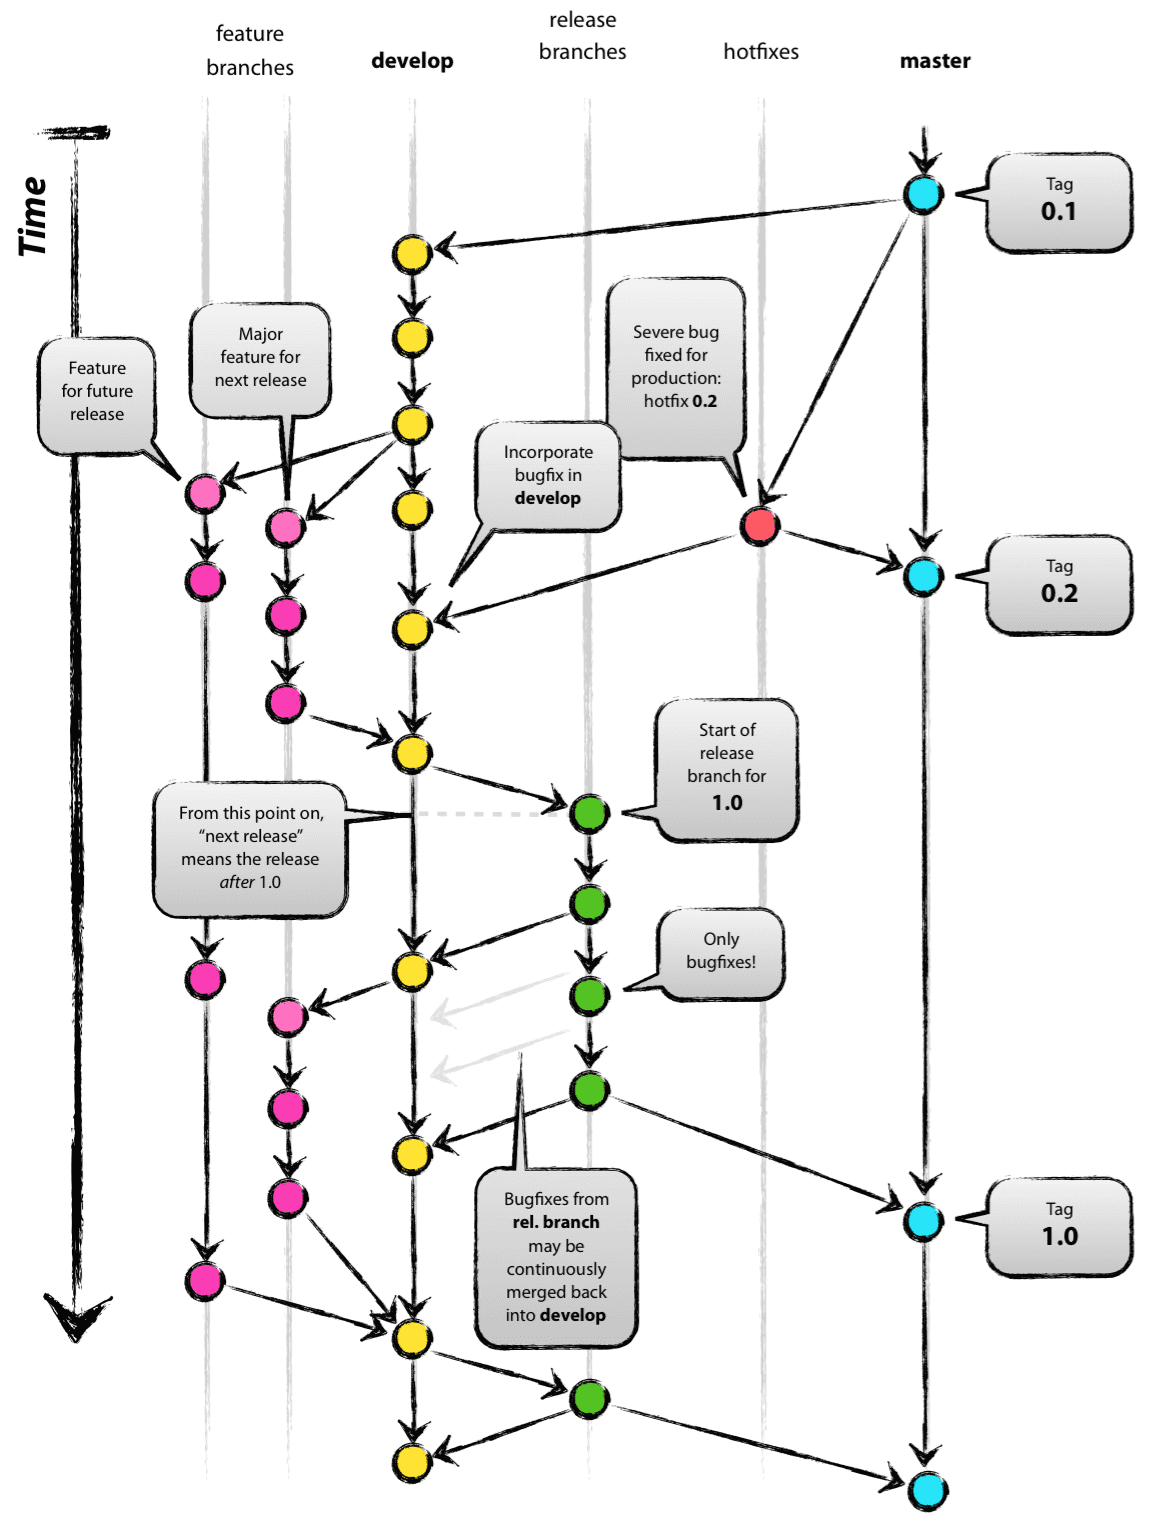
\includegraphics[scale=0.3]{../d/pics/branching.png}
    \caption{Модель разработки}
    \label{fig:branching}
\end{figure}

\newpage

\section{Разработка серверной части}
Несмотря на то, что большинство существующих систем использует реляционные
базы данных, в своем проекте мы решили отказаться от традиционного подхода
к базе данных и использовать, современный, набирающий в последнее время популярность
NoSQL подход. NoSQL решения для управления большими данными используют гиганты индустрии,
такие как: IBM, Facebook, Netflix, EBay, Hulu, Yahoo!, благодаря поддержке которых технология
широко распространилась за последние несколько лет.

В разработке нашего решения для управления проектами мы использовали документоориентированную
систему управления базами данных Apache CouchDB.

Документоориентированные СУБД специально предназначены для хранения иерархических структур
данных (документов). В основе документоориентированных СУБД лежат документные хранилища (англ. document store),
имеющие структуру дерева (иногда леса).

Такой подход очень подходит для построения системы управления проектами, которая тоже имеет древовидную с структуру:
корень дерева --- проект, его узлы --- задачи, пример структуры приведен на рисунке~\ref{fig:project_tree}.

\begin{figure}[!htb]
  \centering
    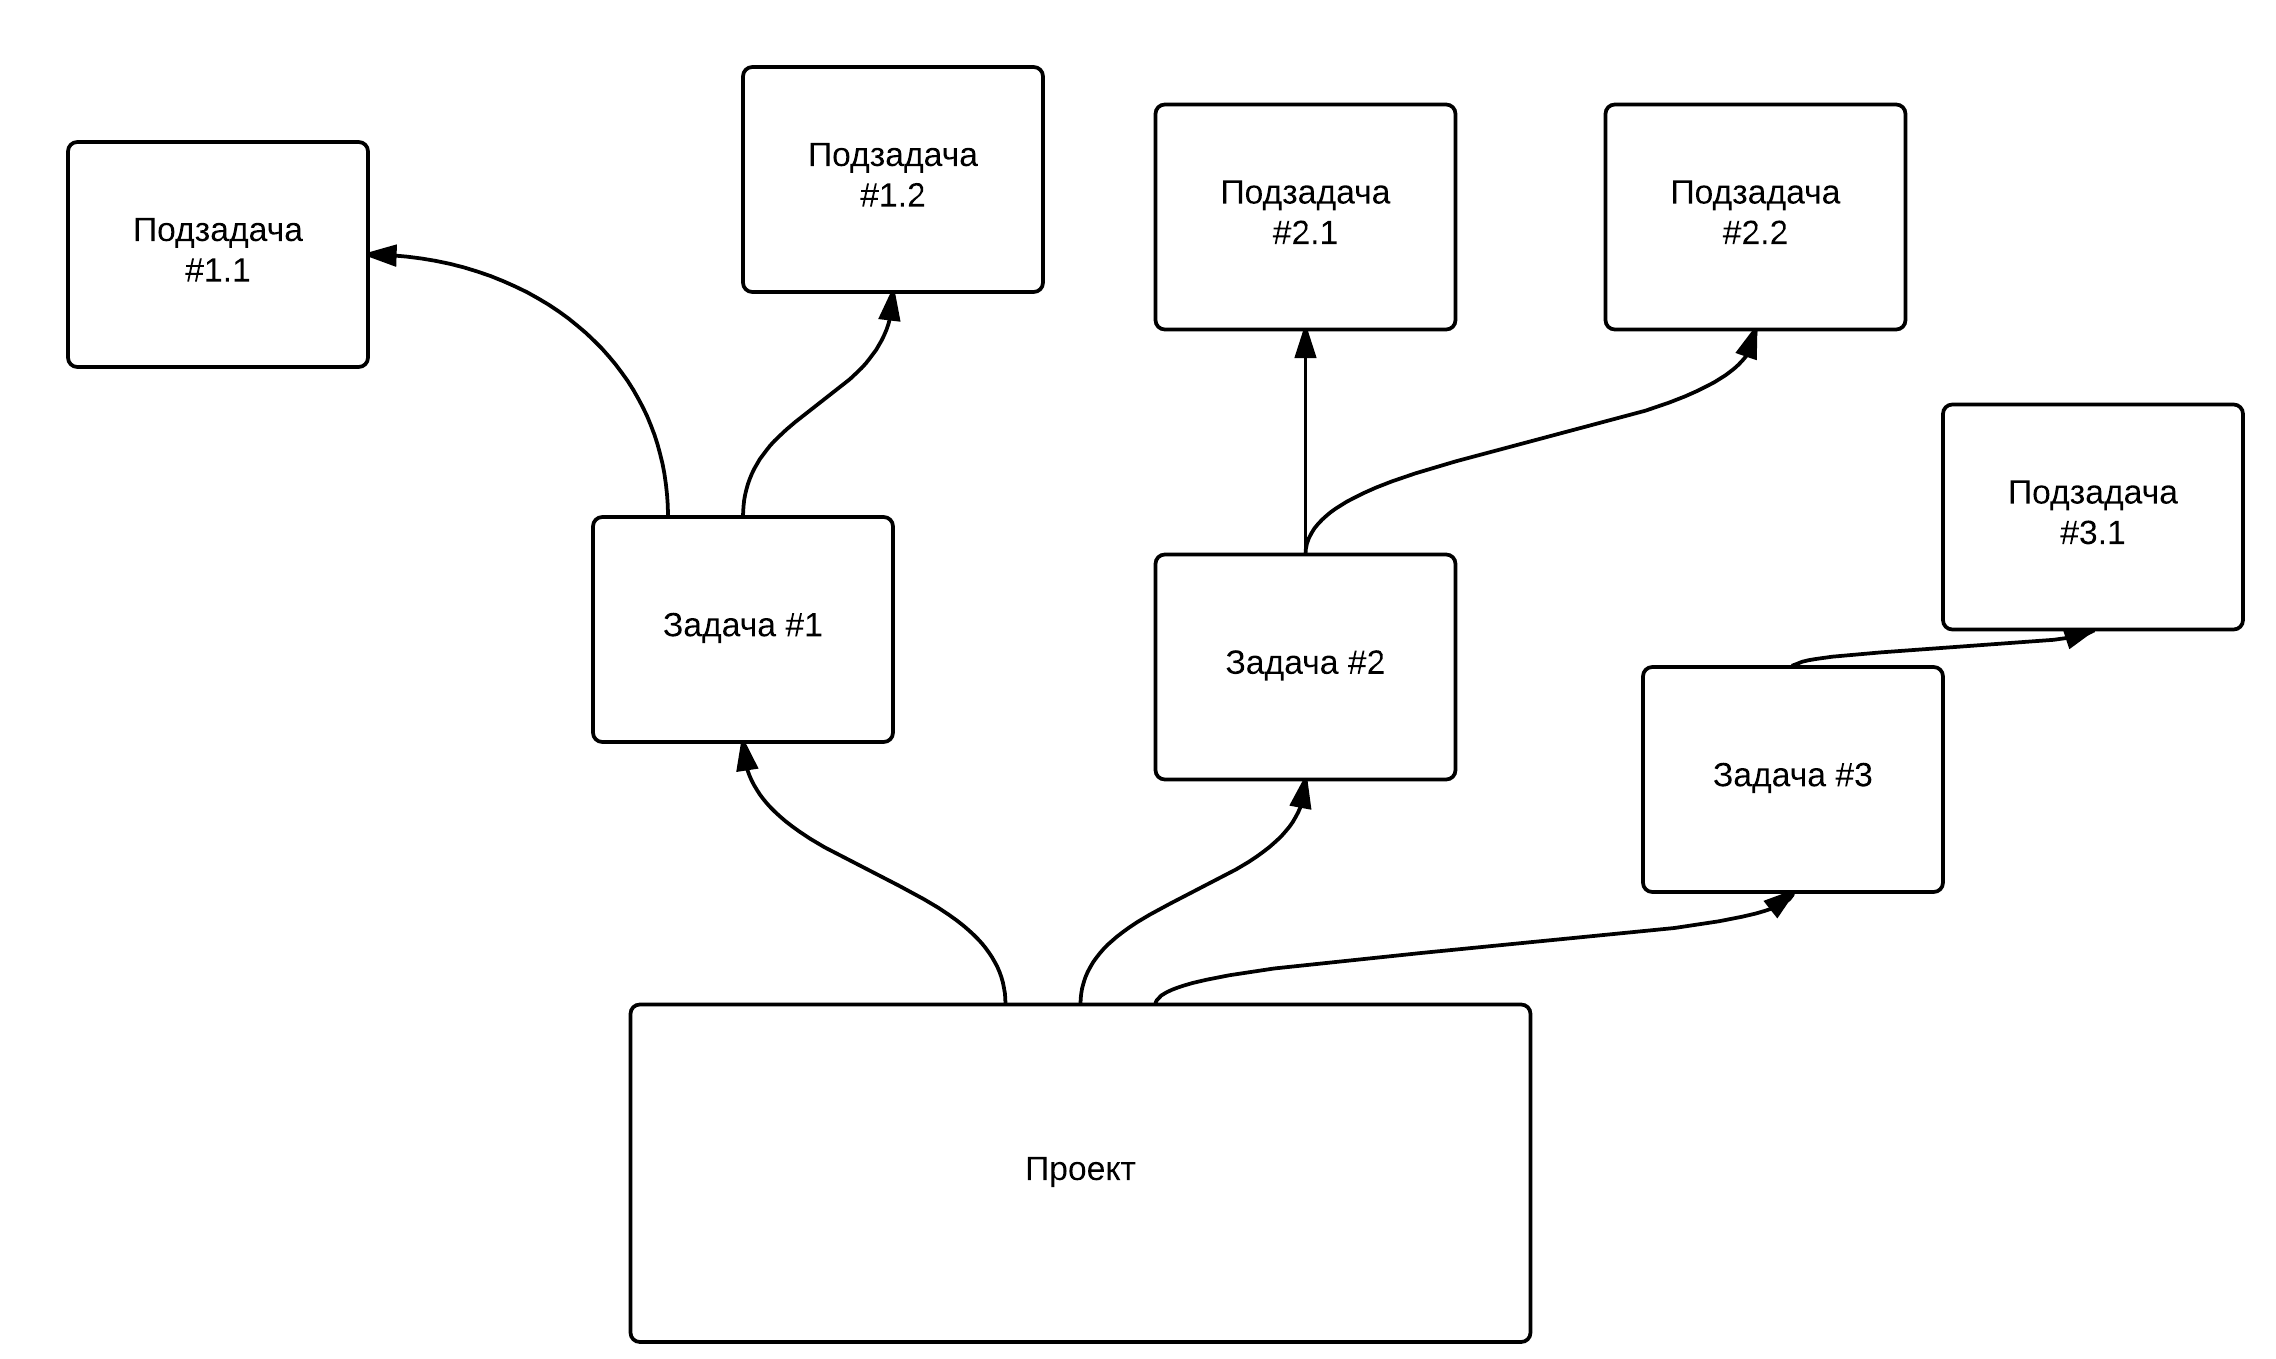
\includegraphics[scale=0.2]{../slides/images/test_tree.png}
    \caption{Структура проекта}
    \label{fig:project_tree}
\end{figure}

Для использования данных из CouchDB в коде приложения мы использовали технологию подобную ORM,
которая связывает базу данных с концепциями объектно-ориентированных языков программирования,
таким образом как бы создавая <<виртуальную объектную базу данных>>.

\newpage


\section{Клиентская часть} % исправить заголовок?

\newpage


\section{Выводы}
% Ещё немного про то, что мы, безусловно, не конкуренты кому-либо, но наш проект можно использовать и вообще!

\newpage


\section{Паспорт проекта}
% Сырые PDF, экспортированные из MS Word; я не хочу перевёрстывать их в TeX
\newpage


\addcontentsline{toc}{section}{Список использованных источников}
\begin{thebibliography}{}
\bibitem{wiki_pm} Электронный ресурс <<Википедия>>: \\https://ru.wikipedia.org/wiki/Управление\_проектами
\bibitem{jira_off} Официальный сайт системы Atlassian JIRA: https://www.atlassian.com/software/jira
\bibitem{redmine_off} Официальный сайт системы Redmine: http://www.redmine.org
\bibitem{bugzilla_off} Описание возможностей на официальном сайте системы Bugzilla: https://www.bugzilla.org/features
\bibitem{wrike_off} Документация на официальном сайте системы Wrike: https://developers.wrike.com/documentation/api/overview
\bibitem{git_home} Домашняя страница Git: http://git-scm.com
\bibitem{git_branching_model} A successful Git branching model By Vincent Driessen: http://nvie.com/posts/a-successful-git-branching-model
\end{thebibliography}

\end{document}
